\documentclass[12pt]{article}
\usepackage[shortlabels]{enumitem}
\usepackage{float}
\usepackage{xcolor}
\usepackage[a4paper, top=1.5cm, bottom=1.5cm, left=2cm, right=2cm]{geometry}
\usepackage{parskip}
\usepackage{setspace}
\usepackage{lmodern}
\usepackage[T1]{fontenc}
\usepackage[brazil]{babel}
\usepackage{hyperref}
\usepackage{graphicx}
\usepackage{amsmath}
\usepackage{amssymb}
\usepackage{amsfonts}
\usepackage{dsfont}

\title{Atividade em Sala - Estatística para Administração - 2025.2}
\date{}

\begin{document}
\maketitle

\section*{Instruções}
\begin{itemize}
    \item Todas as questões a seguir devem ser respondidas em grupo.
    \item \textbf{Não} é permitido fazer esta tarefa sozinho; se você estiver sozinho, procure um grupo. No caso extremo de alguém estar sozinho e não ter nenhum grupo com menos de 4 pessoas,
    é permitido fazer em 5, sendo esse grupo não oficial para o trabalho da disciplina. \textbf{Ninguém} deve fazer esta tarefa sozinho. 
    \item O grupo deve escrever as respostas nas folhas fornecidas, sendo todas as respostas referentes ao grupo, ou seja, \textbf{não} é necessário que cada 
    membro do grupo transcreva as respostas individualmente. 
    \item Não esqueça de escrever o nome dos membros do grupo que fizeram esta tarefa na folha. 
    \item Ao final, entregue suas respostas conjuntamente com o artigo. Vocês podem ficar com as folhas de perguntas como material de estudo para a prova.  
\end{itemize}

\section*{Questão 1}
Leia o seguinte artigo e escreva um comentário acerca da metodologia adotada pelos autores. Adote um posicionamento crítico versando sobre 
o método de amostragem adotado pelos autores. Embase seus argumentos nas discussões realizadas em sala acerca do processo de amostragem. 

\begin{itemize}
    \item Nesta questão, é recomendado que vocês usem o celular para escanear o QR Code abaixo. Quem não tiver celular ou preferir ler no papel,
existem duas cópias físicas do artigo para cada grupo. 
    \item Não existe limite para o tamanho do comentário; o importante é que cada membro do grupo consiga colocar seu posicionamento.
    \item Não precisa ser um texto longo; lembre-se de que existem mais 3 questões nesta tarefa, gerencie eficientemente o tempo.  
\end{itemize}

Link: \url{https://qrco.de/bgIfzU}
\begin{figure}[H]
    \centering
    
\includegraphics[width=0.4\linewidth]{figures/qr_code.png}
\end{figure}





\section*{Questão 2}
Gabriel trabalha no setor de Marketing da empresa Druker S.A. e desconfia que está recebendo um salário menor que os demais colegas de seu setor.
Com o objetivo de verificar tal fato, ele pergunta à Julia, funcionária do setor de Gestão de Pessoas, os salários dos funcionários do setor 
de Marketing da empresa. Julia prontamente responde que trata-se de uma informação sigilosa e que não pode ser fornecida,
mas informa que pode informar medidas de resumo, dizendo em seguida que a média salarial do setor é de R\$ 6.140,00. 

\begin{enumerate}[a)]
    \item Gabriel sabe que seu salário é R\$ 5.900,00. Que informações acerca da distribuição salarial do setor 
    ele pode extrair a partir da informação fornecida por Julia? Gabriel poderia afirmar que está recebendo um salário aproximadamente igual aos dos demais colegas?
    
    No dia seguinte, Gabriel adota a estratégia de perguntar à outra pessoa sobre informações salariais de seu setor.
    Nesse sentido, ele resolve perguntar a sua amiga Amanda, supervisora de Julia, qual seria a mediana dos salários
    do setor de Marketing. Amanda informa que existe uma apresentação interna do setor de Gestão de Pessoas em que são apresentadas medidas de resumo dos salários de cada setor,
    mas que, por se tratar de um documento interno, não pode divulgar. Após ler o documento, Amanda informa que a mediana do salário do setor de Marketing é igual a R\$ 3.750,00.
    
    \item Sabendo agora da mediana, que conclusões Gabriel pode tirar acerca de sua desconfiança em relação ao salário? Que conclusão ele pode tirar a partir do
    fato de a mediana ser menor que a média? 
    
    Mesmo sabendo a média e a mediana salariais, Gabriel está ainda mais curioso em saber a distribuição salarial dos funcionários de seu setor. 
    Então, ele decide sorrateiramente, na hora do almoço, acessar o computador de Daniel, estagiário do setor de Gestão de Pessoas. Gabriel então encontra o documento contendo
    medidas de resumo acerca dos salários do setor de Marketing, verificando que o desvio padrão salarial é igual a R\$ 6.150,00. 
    
    \item Agora, em posse do desvio padrão, a que conclusão Gabriel chega acerca da distribuição salarial dos funcionários do setor de Marketing? 
    
    \item Calcule o coeficiente de variação dos salários do setor de Gabriel; o que podemos afirmar sobre a dispersão dos dados? Qual a conclusão prática?
    
    \item A partir do cenário descrito anteriormente, discuta com seu grupo a seguinte afirmação: Saber a média, a mediana e o desvio padrão é suficiente para conhecer um conjunto de dados. Escrevam um parágrafo acerca das conclusões que vocês chegaram. 
\end{enumerate}

\section*{Questão 3}
Um aluno da disciplina de Estatística decide usar a seguinte métrica como medida de resumo para sua análise exploratória de dados:

\[
\tilde{x} = \dfrac{\sum_{i=1}^n (x_i - \bar{x})}{n}
\]

Mostre, usando o conceito de somatório visto em sala, que, independentemente de $n$ e do conjunto de dados $x_1, x_2, \dots, x_n$, a métrica escolhida pelo aluno sempre resulta em zero.
Faz sentido o aluno adotar essa métrica em sua análise?

\section*{Questão 4}
Um dos jogos da loteria federal que vem se tornando popular ao longo dos últimos anos devido à sua aparente facilidade de ganho é a Lotofácil.
 Diferentemente da tradicional Mega-Sena, na Lotofácil existem apenas 25 números, dos quais, na aposta comum, o jogador
deve marcar 15 números, pagando o valor de R\$ 3,00. O jogador recebe um prêmio relativo à quantidade de acertos; a seguir são listados os prêmios do último sorteio:
\begin{itemize}
    \item Prêmio ao acertar 15 números: R\$ 1.764.882,05
    \item Prêmio ao acertar 14 números: R\$ 1.737,36
    \item Prêmio ao acertar 13 números: R\$ 30,00
    \item Prêmio ao acertar 12 números: R\$ 12,00
    \item Prêmio ao acertar 11 números: R\$ 6,00 
\end{itemize}

A seguir, é apresentada uma imagem do cartão do jogo:

\begin{figure}[H]
    \centering
    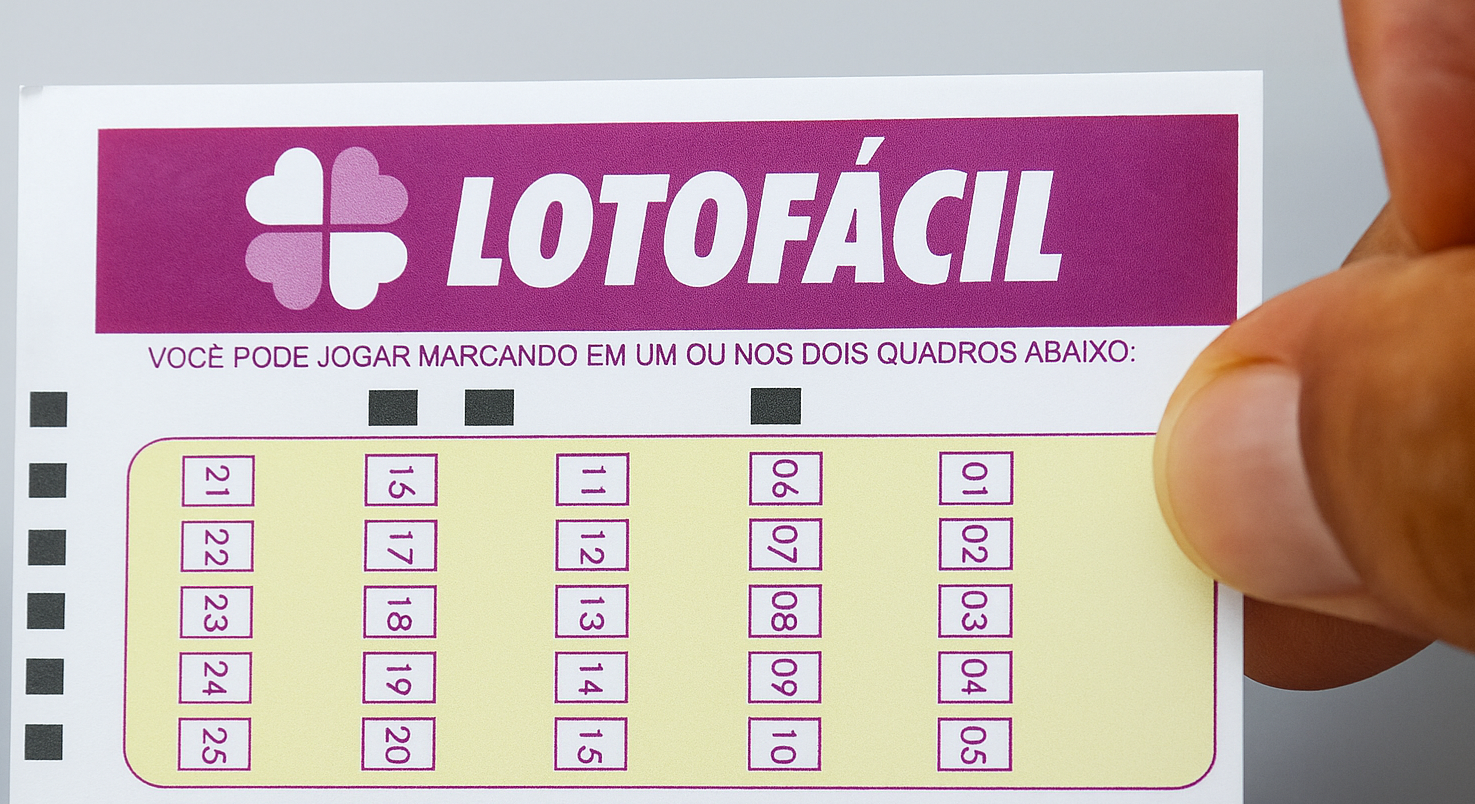
\includegraphics[width=0.5\linewidth]{figures/lotofacil.png}
\end{figure}


Thiago, um jogador da Lotofácil, resolve adotar a seguinte estratégia para aumentar suas chances de ganho: Ele entra na internet e busca todos os números sorteados
    nos sorteios realizados ao longo do ano de 2024 e monta a seguinte tabela de frequência:
\begin{table}[H]
\centering
\caption{Frequência das dezenas da Lotofácil no ano de 2024}
\begin{tabular}{|c|c|c|}
\hline
\textbf{Dezena} & \textbf{Vezes} & \textbf{Frequência Relativa} \\ \hline
10 & 195 & 67,24\% \\ \hline
25 & 191 & 65,86\% \\ \hline
12 & 185 & 63,79\% \\ \hline
02 & 184 & 63,45\% \\ \hline
01 & 181 & 62,41\% \\ \hline
08 & 181 & 62,41\% \\ \hline
04 & 178 & 61,38\% \\ \hline
03 & 177 & 61,03\% \\ \hline
15 & 176 & 60,69\% \\ \hline
20 & 176 & 60,69\% \\ \hline
05 & 175 & 60,34\% \\ \hline
19 & 173 & 59,66\% \\ \hline
07 & 172 & 59,31\% \\ \hline
21 & 171 & 58,97\% \\ \hline
22 & 171 & 58,97\% \\ \hline
23 & 171 & 58,97\% \\ \hline
18 & 170 & 58,62\% \\ \hline
06 & 168 & 57,93\% \\ \hline
13 & 167 & 57,59\% \\ \hline
14 & 166 & 57,24\% \\ \hline
09 & 165 & 56,90\% \\ \hline
24 & 165 & 56,90\% \\ \hline
11 & 164 & 56,55\% \\ \hline
16 & 164 & 56,55\% \\ \hline
17 & 164 & 56,55\% \\ \hline
\end{tabular}
\end{table}

Thiago acredita que a probabilidade de um número ser sorteado está relacionada à frequência com que ele apareceu em sorteios anteriores, ou seja, considera que a probabilidade é proporcional à frequência relativa observada. 
Assim, os números mais frequentes seriam, segundo ele, os mais prováveis de serem sorteados. Dessa forma, com o objetivo de aumentar suas chances de ganhar, ele simplesmente escolhe marcar, no cartão de aposta, os 15 primeiros números da tabela apresentada acima.

Dado esse cenário, responda:

\begin{enumerate}[a)]
    \item Qual interpretação da probabilidade Thiago está usando? 
    \item A interpretação adotada por Thiago é a mais adequada para o contexto do problema? Se a resposta for não, qual seria a interpretação mais adequada e por quê? Se for sim, diga o motivo. 
    \item Discuta as diferenças entre a interpretação clássica e a frequentista da Probabilidade. 
    Discuta o que cada interpretação afirma, evidenciando as principais críticas a cada uma das interpretações e dê exemplos do mundo real nos quais seria mais adequado usar cada uma das abordagens. 
\end{enumerate}  

\end{document}